\documentclass[10pt,letterpaper]{report}
\usepackage[utf8]{inputenc}
%\usepackage{fancyhdr} %para que los capitulos se eliminen
%\renewcommand{\chaptername}{Algo}
\usepackage{titlesec} %esttas doli linas corrigen o quita chapte pero no numeran
\titleformat{\chapter}{}{}{0em}{\bf\LARGE}
\usepackage{amsmath}
\usepackage{amsfonts}
\usepackage{amssymb}
\usepackage{graphicx}
\usepackage[left=2cm,right=2cm,top=2cm,bottom=2cm]{geometry}
%\setlength{\headheight}{25.19998pt}
\usepackage{geometry}
\usepackage{float} %para que no se muevan las tablas
%-------------------------------para uml
%\usepackage{tikz,pgfplots}
%\usetikzlibrary{positioning}
%\usepackage{silence}
%\WarningFilter{pgf}{Your graphic driver} 
%\usepackage{tikz-uml}
%\tikzumlset{fill usecase=white}
%\usepackage{pdflscape}
%----------------------------------------fin uml
\usepackage{appendix}
\usepackage{framed, color}
\usepackage[spanish]{babel}
\usepackage[table]{xcolor}
%\usepackage[linktoc=page]{hyperref} esto hace que no funcione hiperref
\usepackage{advdate}%para que en las tablas se pueda sumar fechas https://tex.stackexchange.com/questions/4873/date-calculations
\usepackage{hyperref}
\hypersetup{
    colorlinks=true,
    linkcolor=black,
    filecolor=magenta,      
    urlcolor=cyan,
    pdfpagemode=FullScreen,
    }

%%%%%%%%%%%%%%%%%%%%%%%%%%%%%%%%%%%%cabecera y pie%%%%%%%%%%%%%%%%%%%%%%%%%%%%%%%%%%%
%\usepackage{fancyhdr, lastpage}
%\pagestyle{fancy}
%\fancyhead{} %limpia cabecera
%\fancyhead[C]{
%\begin{tabular}{|l|l|l|}\hline
%Nombre del proyecto: Biblioteca DP & Version: 1.0 \\ \hline
%Visión:  & Fecha: \today \\ 
%\end{tabular}
%}
%%%%%%%%%%%%%%%%%%pie pagina %%%%%%%%%%%%%%%%%%%%%%%%%%%%%%%%%
%\cfoot{página \thepage\ de \pageref{LastPage}}
%
%%%%%%%%%%%%%%%%%%%%%%%%%%%%%%%%%fin cabecera  y pie %%%%%%%%%%%%%%%%%%%%%%%%%%%%%%%%%%%
\author{TOMÁS ÁLVAREZ DAZA}
\begin{document}

\begin{titlepage}
	\begin{figure}
		
\includegraphics[width=2cm]{images/logoUbi2.png}
	\end{figure}
	\title{PLANIFICACIÓN DEL DESARROLLO DE SOFTWARE\\
	(SISTEMA DE BIBLIOTECA DIGITAL)\\
	Materia:Taller de Sistemas I\\ 
	Docente: Ing. Javier Kanqui\\
	\vspace{1cm}

 \begin{tabular}{c|c|r}
	\hline
	Autor & Versión & Fecha \\
	\hline
	Tomás Álvarez Daza & 1.0 & 21-sep-2022 \\
	\hline
	\end{tabular}}
	
\end{titlepage}
\maketitle

\tableofcontents


%\chapter*{RESUMEN}

El sistema facilita el acceso a todos los recursos llamados aquí  \textbf{documento} que el alumno posee, es decir que ordena y facilita el acceso y satisface la su necesidad de información rápida, ordenada y barata. 

El objetivo que se busca con este sistema es que el alumno se convierta en un individuo independiente con criterio propio mediante el aprendizaje y el conocimiento adecuada y así ayudarse a si mismo en su nivel de vida y en concecuencia a la sociedad. 

El sistema pretende alcanzar a cualquier individuo con necesidad de información con tecnología suficiente para el almacenamiento de su biblioteca personal con sus propios recursos es decir documentos que posee o adquiere en el trenscurso de su carrera y a un menor costo posible. 

El sistema tiene limitaciones ya que no podrá tener toda la bibliografía que tiene una gran biblioteca digital sin embargo podrá ser expansible según a lo que necesite el estudiante y que pueda alimentar al sistema con documento requeridos.
\chapter*{PROBLEMA PRINCIPAL}
%Describe la situación previa al desarrollo de tu software

\section*{INTRODUCCIÓN}
Una biblioteca digital se concibe como una colección organizada de información. La organización es lo que caracteriza a la biblioteca de la world wide web donde hay una anarquia. Además un sitio web tiene que ser editado y actualizado escribiendo y modificando; sin embargo en una bibliteca digital se puede añadir facilmente nuevo material. Además la libreria digital tiene ventajas sobre las convencionales porque son fáciles de acceder y ofrecen busquedas más poderosas.

Las bibliotecas son el repositorio de conocimientos de la humanidad aunque en la antiguedad solo era útil a un pequeño grupo de población. Pero, ahora con la revolución de la información hay una demanda para guardar, organizar y acceso a la información. 

\begin{figure}[ht]
\centering
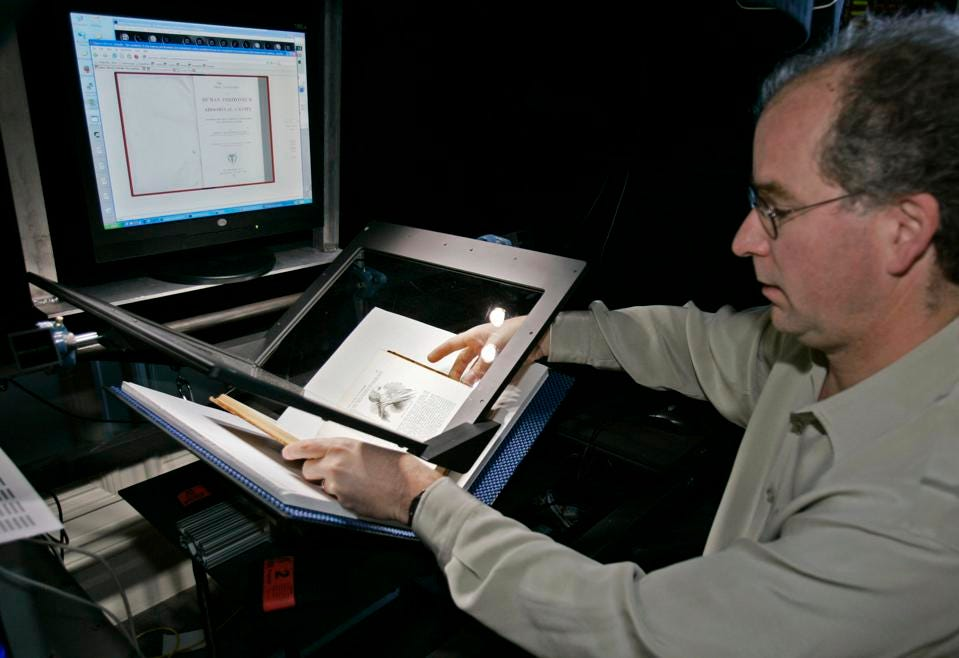
\includegraphics[width=10cm]{images/scaneandoLibro.jpg}
\end{figure} 

\begin{quote}
Goethe dijo una vez que visitar una biblioteca era como entrar en el presencia de una gran rico que silenciosamente estaba pagando dividendos incalculables
\end{quote}
\section*{ANTECEDENTES INSTITUCIONALES}
\subsubsection{Necesidades del software}
Actualmente un estudiante posee los libros digitales o digitalizados y otros como videos, artículos en un disco duro de 2 TB organizado en carpetas sin acceso fácil a ellos. En la actualidad sólo es
posible hacer un link con un programa llamano Kiwix Desktop con el cual es posible acceder con un click al libro en formato pdf o cualquier otro video o artículo o audio (aquí llamados documentos). Este método es inefectivo ya que requiere mucho tiempo para hacer los links.
Los libros están en diferentes formatos como ser: pdf, pub, djvu, pero mayormente en pdf, algunos en html. Actualmente solo se tiene en discos duros y en memoria de dispositivos móviles como tablets, celular o utro dispositivo, muchos ocupan mucha memoria porque hay redundacia de datos ya que una copia está en un disco y otra copia del mismo en otro dispositivo; sin embargo se sugiere tener una copia por si la copia descargada se corrompe.

Las videos, fueron descargados para que tengan buena calidad y sean de latencia mínima alreproducirlos, aunque no se tiene gran cantidad, pero en el futuro esto se incrementará. Los videos se tienen en discos externos; ésto para no sobrecargar el almacenamiento de la computadora personal.
Las imágenes no se tiene mucho, sin embargo como el alumno suele ser más visual en el método de aprendizaje tambien se prevee tener una base de datos de imágenes importante y relevantes a cada tema.

En otros se tiene herramientas como calculadoras, IDEs, CASE, diagramadores y páginas web relacionados con simulación y otros necesarios para aprendizaje.
\subsubsection*{Problemas por la no existencia del software}
El alumno o estudiante tiene mucha información generada durante su paso como estudiante pero éstas estan desorganizadas y el acceso a veces se vuelve de forma que no se puede encontrar lo que se busca. 

Si el alumno tiene ordenado en su computadora cuando se encuentra lejos de donde estudia, no puede acceder y debe llevar copias pero a veces copia un contenido pero tarda en copiar o simplemente copió otro contenido y un sin fin de problemas que puede tener el no accesos oportuno a la información. 

\section*{LIMITES Y ALCANCES DEL SISTEMA}
En primera instancia sólo se desarrollará para documentos tales como artículos y libros, sin embargo para versiones posteriores será extensible a cualquier objeto digital que el alumno requiera para su aprendizaje. 

\section*{JUSTIFICACIÓN}
Un usuario cualquiera requiere como soporte una colección bien articulada de información organizada y estructurada aquí llamados documentos (texto, audio, video es decir un conjunto de objetos digitales, simuladores, etc) para ayudarse un individuo a lograr un objetivo cualquiera y esto no requiere un gran espacio físico. Se quiere realizar esta biblioteca ya que la red de redes carece de caracteristicas esenciales de selección y organización a pesar que pueden existir sitios web con contenido bien organizado la libreria digital puede expandirse facilmente añadiendose nuevo material. Además no a todo el territorio boliviano alcanza la red de redes y ademas si fuera esto posible la velocidad del internet no siempre es alta y que un video pueda ser reprocucido de inmediato y sin latencia de carga y con el dificultad de que buscar algo en internet a veces suele ser como buscar en un pajar. 

Hoy en día con la revulución de la información y el poder de la tecnología hay una demanda sin precedencias para el almacenamiento, organización y acceso a la información y si la información es la moneda de la economia del conocimiento entonces las librerias digitales serán los bancos donde se invierte \cite{91364001}. 

Una biblioteca convencional o en carpetas tiene unas sola forma de organizar, mientras que en una biblioteca digital se puede organizar de diferentes maneras. 

\section*{OBJETIVOS DEL SISTEMA}
El objetivo es realizar el diseño de una herramienta de estudio efectiva para población de diferentes niveles para ayudar en el  proceso de aprendizaje.  
\section*{OBJETIVOS SECUNDARIOS}
\begin{itemize}
	\item Hacer una biblioteca digital más flexible y adaptable posible.
	\item Seleccionar organizar y mantener objetos digitales para el estudiante
\end{itemize}



\part{Requerimientos}
\chapter{LISTA DE REQUERIMIENTOS}
\section{REQUERIMIENTOS FUNCIONALES}
\begin{enumerate}
	\item \textbf{Es accesible via navegador web}
	\item \textbf{permite busqueda por texto a algún campo: }Por ejemplo por palabra clave clave de articulos.
	\item \textbf{Busqueda flexible:} El usuario puede buscar por título, autor, fechas, ectructuras de clasificación, etc. 
	\item \textbf{Hace uso de la metadata disponible: } Para incorporar nuevo material a la biblioteca. 
	\item \textbf{Maneja otro tipo de objetos digitales: } Por ejemplo video, imágens, audio, IDEs, páginas web es dicir links.
	\item Todo lo que ves lo puedes obtener.
	\item El sistema puede funcionar en linea así también de forma local y que el estudiante pueda añadir fácilmente nuevo material a su biblioteca digital. 
	\item El estudiante pueda conectarse de forma remota con su biblioteca digital de cualquier lugar por internet y así también por la red local. 
	\item Debe tener una versión de escritorio para S.O. comunes como Linux/GNU, Window y Mac. 
	\item Que permita clonar todo el sistema y su contenido de forma fácil a un dispositivo de almacenamiento masivo si se desea utilizarlo de forma local (sin internet)
	\item Que puede manejar  de forma automática  la duplicidad de documentos
\end{enumerate}

\section{REQUERIMIENTOS NO FUNCIONALES}
\begin{enumerate}
	\item Debe sorporta multiples descargas al menos hata 20 simultaneamente. 
	\item La seguridad no debe ser tomado en cuenta, puede copiar o clonar el sitema cualquiera que desee si se desea trabajar de forma local. 
	\item Si se accede a la biblioteca por el navegador, el usuario debe estar suscrito. 
	\item Debe ser adaptable a cualquier contenido digital
\end{enumerate}
\section{ESCALABILIDAD} El software debe ser escalable para contener cualquier objeto digital y adecuarse al volumen de almacenamiento.%--------------------------requerimientos
%\part{Plan de desarrollo del proyecto}
%\addcontentsline{toc}{chapter}{CONTROL DE CAMBIOS}
\chapter*{CONTROL DE CAMBIOS}
\stepcounter{chapter}
\begin{table}[h]
\centering
\begin{tabular}{|l|l|p{5cm}|p{4cm}|}\hline
Fecha      &     Versión &    Descripción   &  Autor\\ \hline
\today & 1.0 & Versión preliminar como propuesta de desarrollo & Tomás Álvarez\\ \hline
\AdvanceDate[5]\today & 1.1 & Corrección de diseño de base datos & Tomás Álvarez\\ \hline
\end{tabular}
\end{table}

%
%\ aquí se menciona el proposito, descripción del producto
\addcontentsline{toc}{chapter}{Introducción}
\chapter*{Introducción}
\stepcounter{chapter}
Una vez que es completada los requerimientos del proyecto y los objetivos que es el desarrollo del Sistema Software de Gestión de Farmacia. Con tiempo y presupuesto limitados. En aras de la satisfacción de la cliente se reunió con todos los miembros del proyecto para estructurar los puntos principales y asignación de roles. 

\section{Descripción del proyecto}
Actualmente el estudiante posee los libros digitales o digitalizados y otros como videos, artículos en un disco duro de 2 TB organizado en carpetas sin acceso fácil a ellos. En la actualidad sólo es
posible hacer un link con un programa llamano Kiwix Desktop con el cual es posible acceder con un click al libro en formato pdf o cualquier otro video o artículo o audio (aquí llamados documentos). Este método es inefectivo ya que requiere mucho tiempo para hacer los links. Además cuando se cambia el nombre de la carpeta superior o del mismo se pierde el acceso. 
Los libros están en diferentes formatos como ser: pdf, pub, djvu, pero mayormente en pdf, algunos en html. 
Actualmente se lo tiene en discos duros y en memoria de dispositivos móviles como tablets, celular o utro dispositivo, muchos ocupan mucha memoria porque hay redundacia de datos ya que una copia está en un disco y otra copia del mismo en otro dispositivo y alguno se corrompe al hacer copias y cerrar sin guardar un documento que se estaba viendo .

Las videos, fueron descargados para que tengan buena calidad y sean de latencia mínima al reproducirlos, aunque no se tiene gran cantidad, pero en el futuro esto se incrementará. Los videos se tienen en discos rígidos externos; ésto para no sobrecargar el almacenamiento de la computadora personal.
En cuanto a imágenes no se tiene mucho, sin embargo como el alumno suele ser más visual en el método de aprendizaje también se provee tener una base de datos de imágenes importantes y relevantes a cada tema.

En otros, se tiene herramientas como calculadoras, IDEs, CASE, diagramadores y páginas web relacionados con simulación y otros necesarios para aprendizaje del estudiante, están desorganizados y el alumno pierde buscando lo que una vez ya había encontrado en la web. 
\section{Necesidades del proyecto}
El alumno o estudiante tiene mucha información generada durante su paso como estudiante pero éstas están desorganizadas y el acceso a veces se vuelve de forma que no se puede encontrar lo que se busca. También si el alumno tiene ordenado algo en su computadora, cuando se encuentra lejos de donde estudia, no puede acceder y debe llevar copias pero a veces copia un contenido que tarda en copiar,  o simplemente copió otro contenido y un sin fin de problemas que puede tener el no accesos oportuno a la información. 
%\section{Abreviaturas}
\section{Propósito u objetivo}
El objetivo es realizar el desarrollo de una herramienta de estudio efectiva para población de diferentes niveles para ayudar en el  proceso de aprendizaje.  
Y los objetivos específicos son:
\begin{itemize}
	\item Hacer una biblioteca digital más flexible y adaptable posible.
	\item Seleccionar organizar y mantener objetos digitales para el estudiante
\end{itemize}

\section{Alcance}
En primera instancia sólo se desarrollará para documentos tales como artículos y libros, sin embargo para versiones posteriores será extensible a cualquier objeto digital que el alumno requiera para su aprendizaje. 
\addcontentsline{toc}{chapter}{Vista general del proyecto}
\chapter*{Vista general del proyecto}
\stepcounter{chapter}
%El proyecto de FARMAKUM incluye el desarrollo de software AdmiFarm, un sistema de inventario y facturación alojado en la nube. Admifarm provee los requisitos de comunicación segura
El proyecto de biblioteca digital incluye el desarrollo de software Biblioteca2295 con un sistema de inventario alojado en la nube.
\section{Suposiciones y restricciones}
%Pasos para control de proyecto
\addcontentsline{toc}{chapter}{Organización del Proyecto}
\chapter*{Organización del Proyecto}%19.2.1 Project Organization
El proyecto se organiza con personas que tienen algún conocimientos a cerca de bibliotecas digitales, se busca también algunos con habilidades específicas. 

\stepcounter{chapter}

\section{Participantes en el proyecto}
%https://monday1006.monday.com/boards/3478543214  aquí se puede hacer una tabla
\subsection{Jefe de proyecto} Es el que se encargará del coordinar con todos y ser puente entre el cliente y el equipo.
\subsection{Analista de sistemas} 
Se encarga del modelado funcional, estructural y de comportamiento.
Realiza el modelado de procesos, modelos físico y lógicos (diagrama de casos de uso) 
\subsection{Diseñador  de sistemas} 
Se ocupa de validación, análisis de modelos, estrategias de diseño, como ser el diseño orientado a objetos, capas, interacción computadora-humano y de capa de arquitectura física. 
\subsection{Desarrolladores}
Los desarrolladores se harán cargo de las tecnologías de implementación, crear clases y objetos. También se hacen cargo de manejo de datos y verificación de software. 
\subsection{Tester}
Se encargarán de la calidad de software, proceso de pruebas, pruebas dinámicas y estáticas e implementar herramientas de testeo.
\section{Roles y responsabilidades}
%Tabla con posicion y rol o responsabilidad
\begin{table}
\begin{tabular}{ll} \vline
Posición & Responsabilidad o Rol \\ \vline
\end{tabular}
\end{table}

\addcontentsline{toc}{chapter}{Gestión de proceso}
\chapter*{Gestión de proceso}
\stepcounter{chapter}
%en ingles gestion es management
\section{Estimación del proyecto}
%Faces de desarrollo
%Objetivos
%Plan de despliegue o liberación
%\subsection{Estimación y gestión de recursos humanos}
%\subsection{Estimación de recursos de software}
%\subsection{Estimación del tiempo}
\section{Herramientas para gestión y ciclo de vida de software de proyectos}
\subsection{Herramientas de control de código fuente}
Se utilizará el git como software de control de versiones. 

Se utilizará GitHub como alojamiento de código y de repositorio.
\section{Plan de proyecto}
\subsubsection{Calendario de proyecto}
\subsubsection{Diagrama de Gantt}
%https://www.teamgantt.com/

\section{Seguimiento y control de proyecto}
%\chapter*{Documentación}





\part{Analisis del sistema} %--------------------------Analisis
\chapter*{DIAGRAMA DE PROCESOS}
En este diagrama tratamos de organizar para mejorar como se pueden hacer para beneficial a a las partes interesadas. Se muestra lo que requiere un usuario, en este caso es recopilar documentación que piensa que requiere, recomendación de sus docentes para luego obtener un resultado según a los documentos u objetos digitales que pueda alimentar a la biblioteca. 
\begin{figure}[ht]
	\centering
	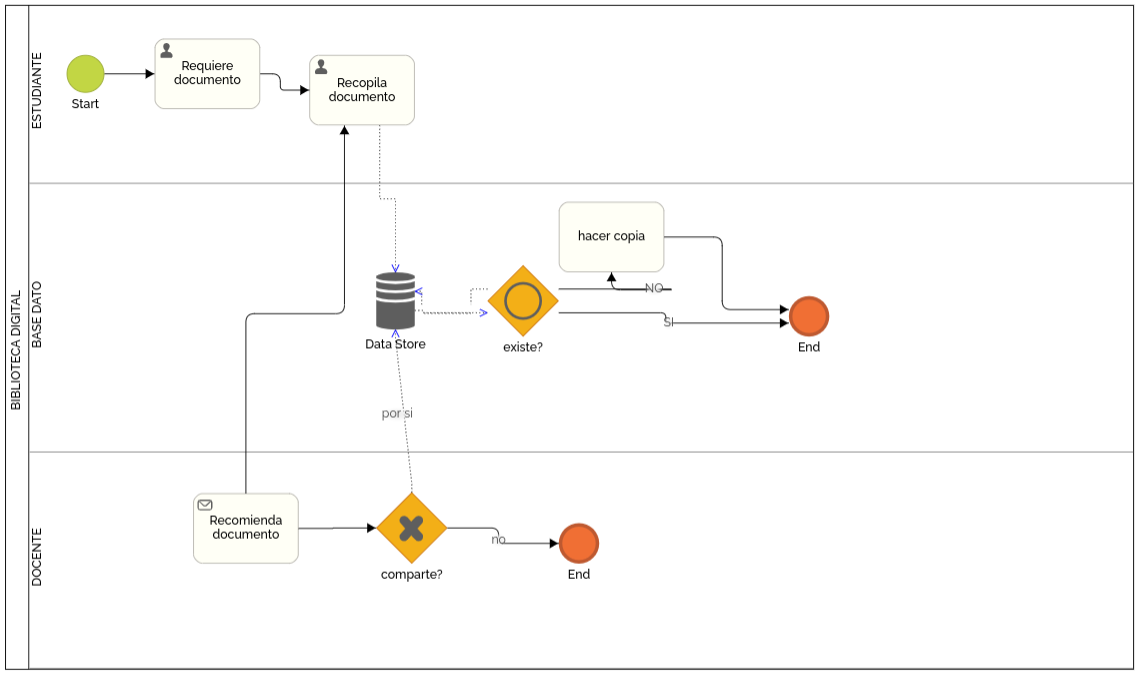
\includegraphics[scale=0.5]{images/modeladoProceso1}
	\caption{Modelado de proceso de la biblioteca digital}
\end{figure}
\chapter*{DIAGRAMA DE CASOS DE USO}

\rowcolors{2}{gray!10}{gray!40}



\begin{figure}[ht]
	\centering
	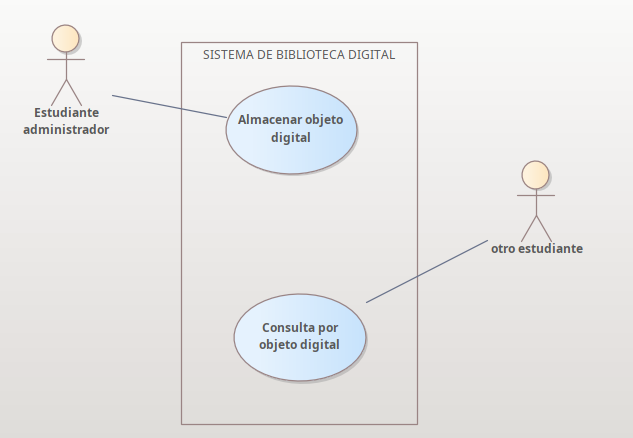
\includegraphics[scale=0.8]{images/casoUso2}
	\caption{Diagrama de casos de uso}
\end{figure}
\begin{center}
\begin{tabular}{lp{10cm}}
    Id del caso de uso & CU-1 \\
    \hline
    Caso de uso & Almacenar objeto digital \\
    Actores & Estudiante administrador \\
    Descripción & Almacena cualquier documento o objeto digital como libros, artículos, videos, audio para poder almacenar un objeto digital (documento o multimedia)  \\
    Precondición & Usuario ingresa al sistema de forma remota, local o por navegador \\
    Post condición & Almacenamiento actualizado \\
\end{tabular}\\
\vspace{0.5cm}
\begin{tabular}{lp{10cm}}
    Id del caso de uso & CU-2 \\
    \hline
    Caso de uso & Consultar por un objeto digital \\
    Actores & Otro estudiante \\
    Descripción & Consulta por cualquier documento o objeto digital como libros, artículos, videos, audio  \\
    Precondición & El estudiante bebe ingresar al sistema\\
    Post condición & Necesidad de información satisfecha \\
\end{tabular}
\end{center}


%---------------------------Diseño
\part{Diseño}
\chapter*{DIAGRAMA DE CLASES}
\begin{figure}[h]
	\centering
	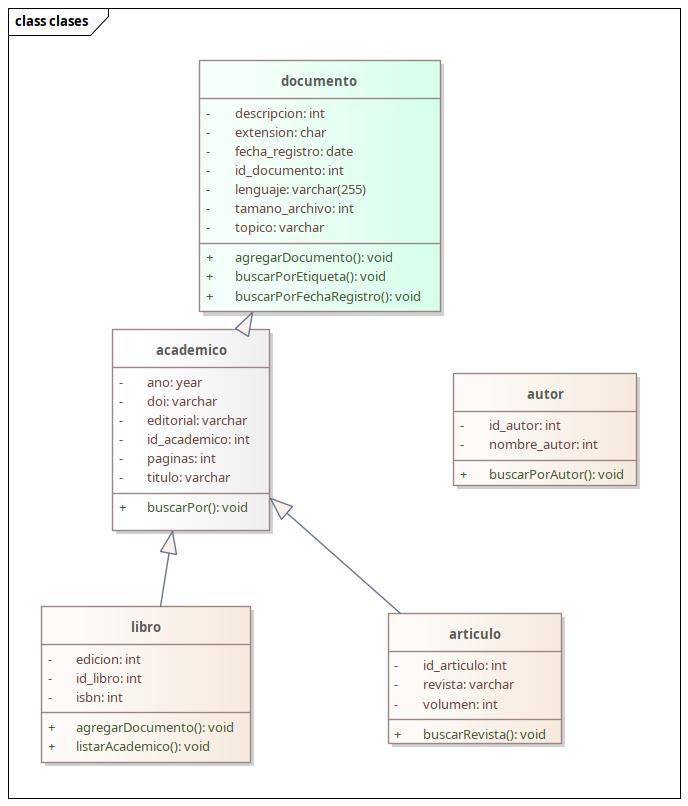
\includegraphics[scale=0.6]{images/clase}
	\caption{Diagrama de clases }
\end{figure}
\chapter*{DIAGRAMA DE SECUENCIA}

\begin{figure}[ht]
	\centering
	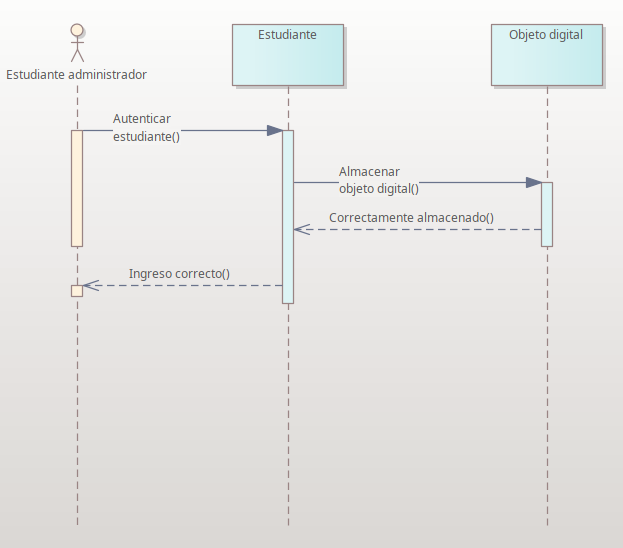
\includegraphics[scale=0.8]{images/secuencia1.png}
	\caption{Diagrama de secuencia}
\end{figure}

\begin{figure}[ht]
	\centering
	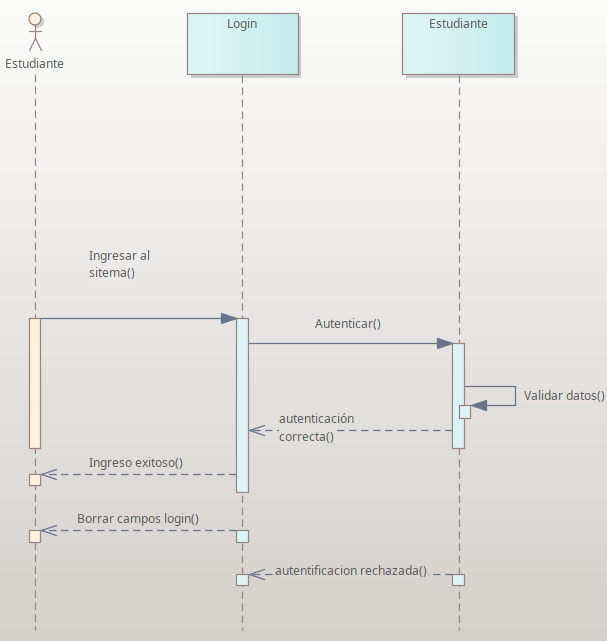
\includegraphics[scale=0.8]{images/secuencia2.png}
	\caption{Diagrama de secuencia para que el estudiante se autentique en el sistema}
\end{figure}

\addcontentsline{toc}{chapter}{Diseño de base de datos}
\chapter*{Diseño de base de datos}
\stepcounter{chapter}
\section{Diagrama entidad relación}
Se abstrae del problema real. Nuestras entidades serán el autor, 
Para el diseño entidad relación de base datos se utiliza la herramienta \textit{Draw io}. 

%\section{MODELO VISTA CONTROLADOR}
%\subsection{MODELO}
%Mapeamos una clase con cada tabla, aquí unimos el código con la base de datos. 
%\subsection{VISTA}
%Aquí está la interfaz
%\subsection{CONTROLADOR}
%%También ya hay el paradigma de microservicios para construir el software
%\section{TECNOLOGÍA ORM UTILIZADO EN EL PROYECTO}
%\subsection{SPRING BOOT}
%%para node se usa express, para php láravel
\section{Diccionario de datos}
% inicia dic datos%%%%%%%%%%%%%%%%%%%


\begin{table}[h]
\resizebox{\columnwidth}{!}{%
\begin{tabular}{llll}
\hline
\multicolumn{3}{l}{\textbf{Nobre del archivo:} Libro}            & \textbf{Fecha de creación:} \today                  \\ \hline
\multicolumn{4}{l}{\textbf{Descripción:} Es un archivo para almacenar libros}                                                                 \\ \hline
\rowcolor[HTML]{C0C0C0} 
\multicolumn{1}{c}{\cellcolor[HTML]{C0C0C0}\textbf{Campo}} &
  \multicolumn{1}{c}{\cellcolor[HTML]{C0C0C0}\textbf{Tamaño}} &
  \multicolumn{1}{c}{\cellcolor[HTML]{C0C0C0}\textbf{Tipo de dato}} &
  \multicolumn{1}{c}{\cellcolor[HTML]{C0C0C0}\textbf{Descripción}} \\ \hline
IDE                    & 6               & Numérico        & Clave única de registro de documento         \\
Año            & 100             & Caracter        & Año del libro                        \\
Editorial              & 10              & Caracter        & hggdg             \\
Edicion             & 5               & Caracter        & Extensión del documenten ej. pdf, upub, djvu \\
Págginas            & 6               & Numérico        & Número de páginas que tiene el libro         \\ \hline
\multicolumn{2}{l}{\textbf{Relaciones:}} & \multicolumn{2}{l}{\textbf{Campos clave:} ID documento}                     \\
\multicolumn{2}{l}{}                     & \multicolumn{2}{l}{}                                           \\ \hline
\end{tabular}%
}
\end{table}

\begin{table}[h]
\resizebox{\columnwidth}{!}{%
\begin{tabular}{llll}
\hline
\multicolumn{3}{l}{\textbf{Nombre del archivo:} Artículo}            & \textbf{Fecha de creación:} \today                  \\ \hline
\multicolumn{4}{l}{\textbf{Descripción:} Contiene }                                                                 \\ \hline
\rowcolor[HTML]{C0C0C0} 
\multicolumn{1}{c}{\cellcolor[HTML]{C0C0C0}\textbf{Campo}} &
  \multicolumn{1}{c}{\cellcolor[HTML]{C0C0C0}\textbf{Tamaño}} &
  \multicolumn{1}{c}{\cellcolor[HTML]{C0C0C0}\textbf{Tipo de dato}} &
  \multicolumn{1}{c}{\cellcolor[HTML]{C0C0C0}\textbf{Descripción}} \\ \hline
IDE                    & 6             & Numérico        & Clave única de registro de documento         \\
DOI                 & 20               & Caracter        & Es un identificador único que nunca cambia asignado a un artículo.             \\
Revista               & 100            & Caracter        & Nombre de revista quien publicó    \\ \hline
\multicolumn{2}{l}{\textbf{Relaciones:}} & \multicolumn{2}{l}{\textbf{Campos clave:} ID documento}                     \\
\multicolumn{2}{l}{}                     & \multicolumn{2}{l}{}                                           \\ \hline
\end{tabular}%
}
\end{table}


\begin{table}[h]
\resizebox{\columnwidth}{!}{%
\begin{tabular}{llll}
\hline
\multicolumn{3}{l}{\textbf{Nombre del archivo:} SitiosWeb}            & \textbf{Fecha de creación:} \today                  \\ \hline
\multicolumn{4}{l}{\textbf{Descripción:} Guarda datos de enlaces a páginas web útiles al estudiante}                                                                 \\ \hline
\rowcolor[HTML]{C0C0C0} 
\multicolumn{1}{c}{\cellcolor[HTML]{C0C0C0}\textbf{Campo}} &
  \multicolumn{1}{c}{\cellcolor[HTML]{C0C0C0}\textbf{Tamaño}} &
  \multicolumn{1}{c}{\cellcolor[HTML]{C0C0C0}\textbf{Tipo de dato}} &
  \multicolumn{1}{c}{\cellcolor[HTML]{C0C0C0}\textbf{Descripción}} \\ \hline
IDE                    & 6         & Numérico        & Clave única de registro del link         \\
URL                 & 20           & Caracter        & URL del enlace a página web             \\
Fecha de acceso     & -            & Fecha           & Fecha en que se guardó el enlace    \\ \hline
\multicolumn{2}{l}{\textbf{Relaciones:}} & \multicolumn{2}{l}{\textbf{Campos clave:} ID documento}                     \\
\multicolumn{2}{l}{}                     & \multicolumn{2}{l}{}                                           \\ \hline
\end{tabular}%
}
\end{table}

\begin{table}[h]
\resizebox{\columnwidth}{!}{%
\begin{tabular}{llll}
\hline
\multicolumn{3}{l}{\textbf{Nombre del archivo:} Autor}            & \textbf{Fecha de creación:} \today                  \\ \hline
\multicolumn{4}{l}{\textbf{Descripción:} Datos del autor}                                                                 \\ \hline
\rowcolor[HTML]{C0C0C0} 
\multicolumn{1}{c}{\cellcolor[HTML]{C0C0C0}\textbf{Campo}} &
  \multicolumn{1}{c}{\cellcolor[HTML]{C0C0C0}\textbf{Tamaño}} &
  \multicolumn{1}{c}{\cellcolor[HTML]{C0C0C0}\textbf{Tipo de dato}} &
  \multicolumn{1}{c}{\cellcolor[HTML]{C0C0C0}\textbf{Descripción}} \\ \hline
IDE                    & 6         & Numérico        & Clave única de registro del link         \\
Nombre                 & 20        & Caracter        & Es el nombre del autor             \\
Pais de origen         & 20        & Caracter        & Pais del autor \\ \hline
\multicolumn{2}{l}{\textbf{Relaciones:}} & \multicolumn{2}{l}{\textbf{Campos clave:} ID documento}                     \\
\multicolumn{2}{l}{}                     & \multicolumn{2}{l}{}                                           \\ \hline
\end{tabular}%
}
\end{table}

\addcontentsline{toc}{chapter}{DISEÑO DE FORMULARIO Y REPORTES}
\chapter*{Diseño de formularios y reportes}
\stepcounter{chapter}
Los formulario serán utilizados tanto para entradas o salida, así también los reportes para transmitir información sobre una colección de datos. El diseño de los formularios y reportes serán la clave para que este sistema sea exitoso. La información es recolectado y formateado de diferentes formas. 
\section{Diseño de Salida efectiva}
La salida es rápida ya que no todos los datos están almacenados en la máquina local y los datos no requieren un procesamiento complejo si se trabaja de forma local. La salida sera preferentemente en pantalla pero se podrá imprimir  si se requiere algún reporte de los libros almacenados. 

La salida facilita al usuario a encontrar lo que realmente busca de manera útil y fácil dependiendo de sus datos o objetos digitales almacenados. Los documentos de pueden abrir con diferentes aplicaciones, reproductores o visualiza dores si es un multimedia. Cambien se puede localizar la dirección donde el objeto está almacenado. 

\begin{figure}[ht]
	\centering
	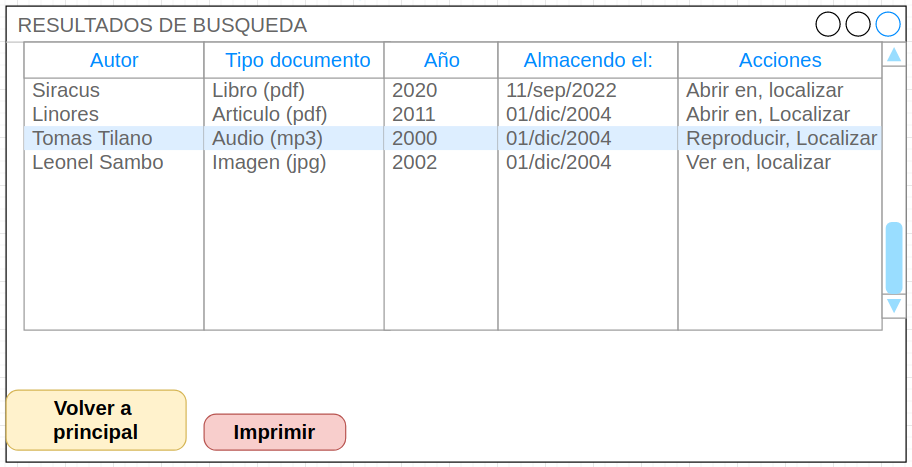
\includegraphics[scale=0.50]{images/resultadoBusqueda1}
	\caption{Resultado ¨de la busqueda}
\end{figure}

\begin{figure}
	\centering
	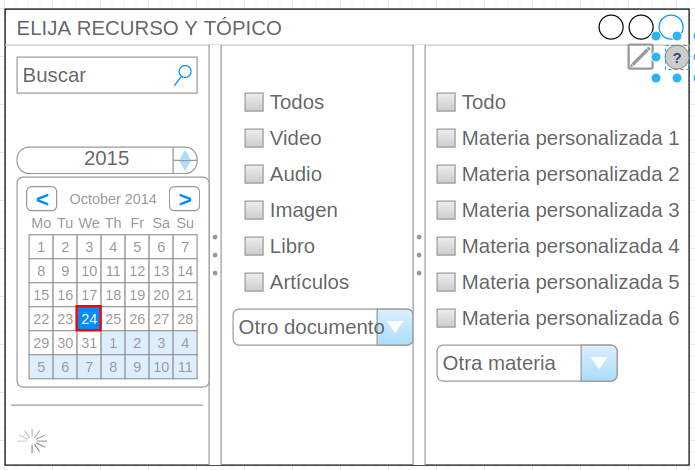
\includegraphics[scale=0.5]{images/buscador1}
	\caption{Pantalla principal de busqueda}
\end{figure}


\section{Diseño de Entrada efectiva}
El ingreso es mayormente de forma automática usando los metadatos de los objetos. 
\begin{figure}
	\centering
	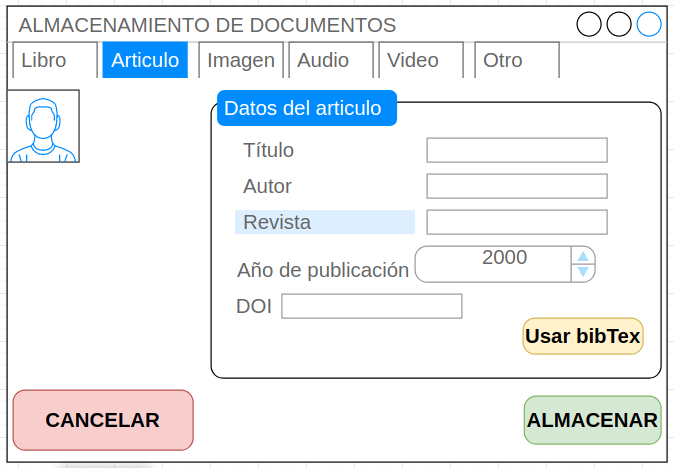
\includegraphics[scale=0.5]{images/almacenamientoDato1}
	\caption{Almacenamiento de artículos}
\end{figure}

%Un \textbf{reporte} es un docomento de negocios que contiene unicamente un dato predefinido.




%------------------------------------IMPLEMENTACION
\part{Implementación}% aqui  paradigam: Microser nosotros API rest
\addcontentsline{toc}{chapter}{Tecnologías}
\chapter*{TECNOLOGIAS}
Para la implementación se utiliza las siguientes tecnología:
\begin{itemize}
\item \textbf{Gestor de dependencias}, MVN
\item \textbf{Lenguaje de programación}, JAVA 17
\item \textbf{Framework}, Spring Boot
\item \textbf{IDE}, GetBrain IDEA
\end{itemize}
Además de otros se expone continuación éstas tecnologías:
\addcontentsline{toc}{chapter}{MAVEN}
\chapter*{MAVEN}
\stepcounter{chapter}
%Aqui usaremos paradigma de micro servicio en nuestro caso api rest
\section{MVN}
Apache Maven es una herramienta de comprensión y gestión de proyectos de software. Basado en el concepto de un modelo de objetos de proyecto (POM), Maven puede administrar la construcción, los informes y la documentación de un proyecto desde una pieza central de información. Se descarga de la siguiente dirección  \url{https://maven.apache.org/download.cgi}, se instala y se verifica como sigue
\begin{verbatim}
tomas@debian:~$ mvn --version
Apache Maven 3.6.3
Maven home: /usr/share/maven
Java version: 17.0.4, vendor: Debian, runtime: /usr/lib/jvm/java-17-openjdk-amd64
Default locale: en_GB, platform encoding: UTF-8
OS name: "linux", version: "5.10.0-19-amd64", arch: "amd64", family: "unix"
\end{verbatim}
\begin{figure}[h]
\centering
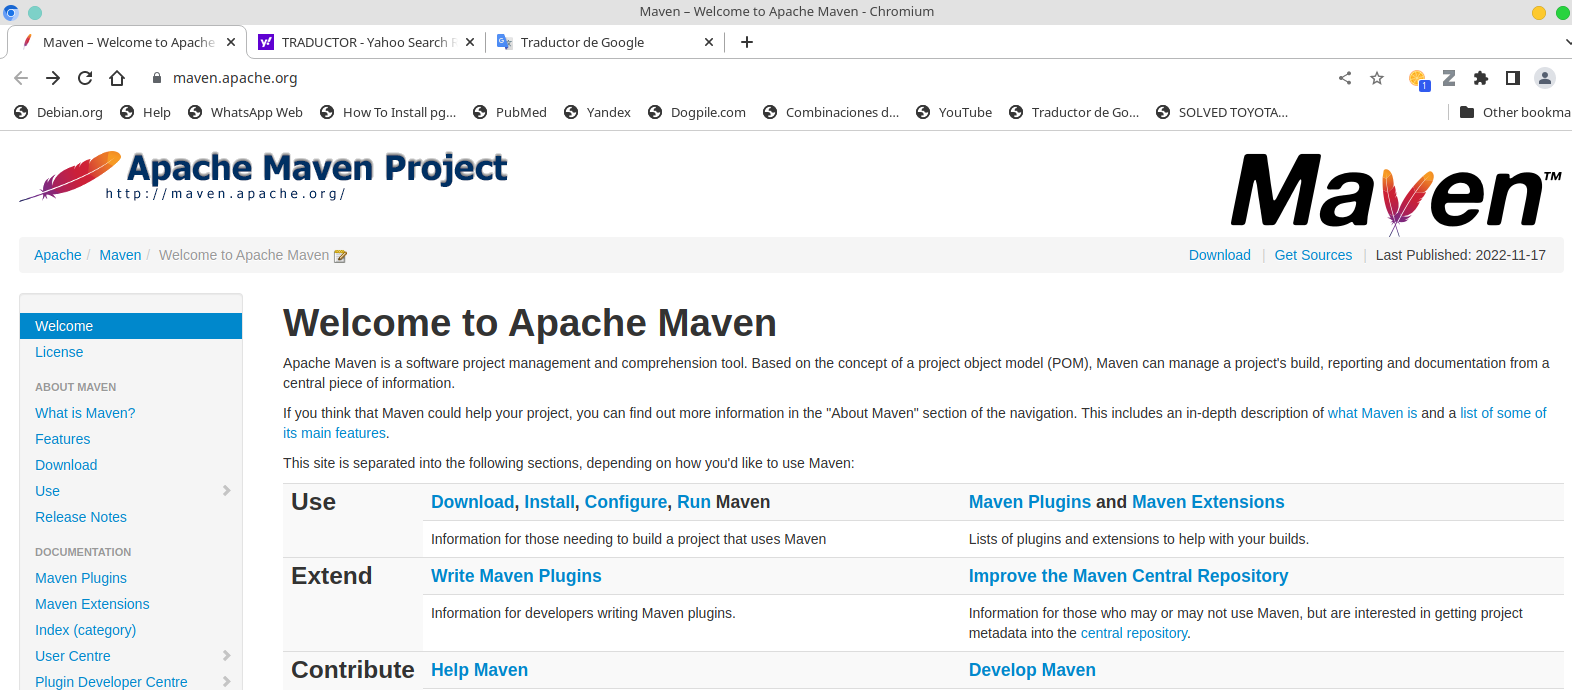
\includegraphics[scale=0.4]{images/maven1}
\caption{Página principal de maven}
\end{figure}
Se debe descara el binario comprimido en .tar (tape archiv); en window se puede descargar lo que puedes descomprimir (generalmente .zip). En windows se descomprime y se configura la carpeta binaria en los variable de entorno. 
\subsection{PROJECT OBJECT MODEL (POM)}
Es un xml  que contiene información a cerca del proyecto y configuración usado por Maven para compilar el proyecto. Project Object Model o POM es la parte básica de la funcionalidad de Maven. Este es un archivo XML que tiene información sobre las dependencias, configuraciones y otra información importante sobre el proyecto. Maven revisa esta información y luego realiza la tarea designada.

Spring Initializr es una API \footnote{ interfaz de programación de aplicaciones API es una forma en que dos o más programas de computadora se comunican entre sí. Es un tipo de interfaz de software que ofrece un servicio a otras piezas de software} que permite la generación de proyectos con sus dependencias permitiendo simplificar esta etapa inicial de arranque de nuevos proyectos. 
%\addcontentsline{to}{chapter}{}
\chapter{JAVA}
%\stepcounter{chapter}
Fue desarrollado por el equipo liderado por James Gosling en Sun Microsystems. Sun microsystems fue comprado por Oracle en 2010. Originalmente llamado Oak, Java fue diseñado en 1991 para uso embebido de chips en electrodomésticos de consumo. En 1995, renombrado Java, fue re diseñado para desarrollo de aplicaciones Web. 

Java se volvió enormemente popular. Fue descrito por sus diseñadores como \textit{ simple, orientado a objetos, distribuido, interpretado, robusto, seguro, neutral arquitecture, portable, de alto rendimiento, multiproceso y dinámico}.

Ahora Java es muy popular para desarrollo de aplicaciones en Servidores Web. Éstas aplicaciones procesan datos, realizan cálculos, y generan páginas web dinámicas. Muchos sitios web comerciales son desarrollados usando java en el backend. 

Java bien es 3 ediciones: \textit{Standard Edition, java Enterprise Edition (Java EE), y Java Micro Edition (Java ME)}. Además éstos están en diferentes ediciones.

\textit{ Java EE} Es para desarrollar aplicaciones en el lado del servidor, tales como Java servlets, páginas JavaServer (JSP), y JavaServer Faces (JSF).

\section{JDK}
Consiste de un conjunto de programas separados. El JDK está en su versión 19 en el momento actual pero LTS es la versión 17 \cite{historia}. 

\section{Versión de java que se utiliza en el proyecto}
\begin{verbatim}
tomas@debian:~$ java --version
openjdk 17.0.4 2022-07-19
OpenJDK Runtime Environment (build 17.0.4+8-Debian-1deb11u1)
OpenJDK 64-Bit Server VM (build 17.0.4+8-Debian-1deb11u1, mixed mode, sharing)
\end{verbatim}








%\addcontentsline{toc}{chapter}{}
\chapter{MySql/Mariadb}
\stepcounter{chapter}
MariaDB es una bifurcación de MySQL impulsada por la comunidad que Monty inició en 2009 Widenius, el autor original de MySQL, después de que Oracle adquiriera el antiguo proyecto.
La primera versión de MariaDB se basó en MySQL 5.1 y las mejoras a El código base de MySQL se fusiona regularmente en el proyecto MariaDB. Otras características
también se fusionan desde Percona Server\footnote{Percona Server for MySQL® es un reemplazo gratuito, totalmente compatible, mejorado y de código abierto para cualquier base de datos MySQL. Proporciona un rendimiento superior, escalabilidad e instrumentación.}, otra bifurcación que es muy similar a la producto principal.

Se utiliza el la siguiente versión:
\begin{verbatim}
Welcome to the MariaDB monitor.  Commands end with ; or \g.
Your MariaDB connection id is 31
Server version: 10.5.15-MariaDB-0+deb11u1 Debian 11
Copyright (c) 2000, 2018, Oracle, MariaDB Corporation Ab and others.
\end{verbatim}

\begin{figure}[h]
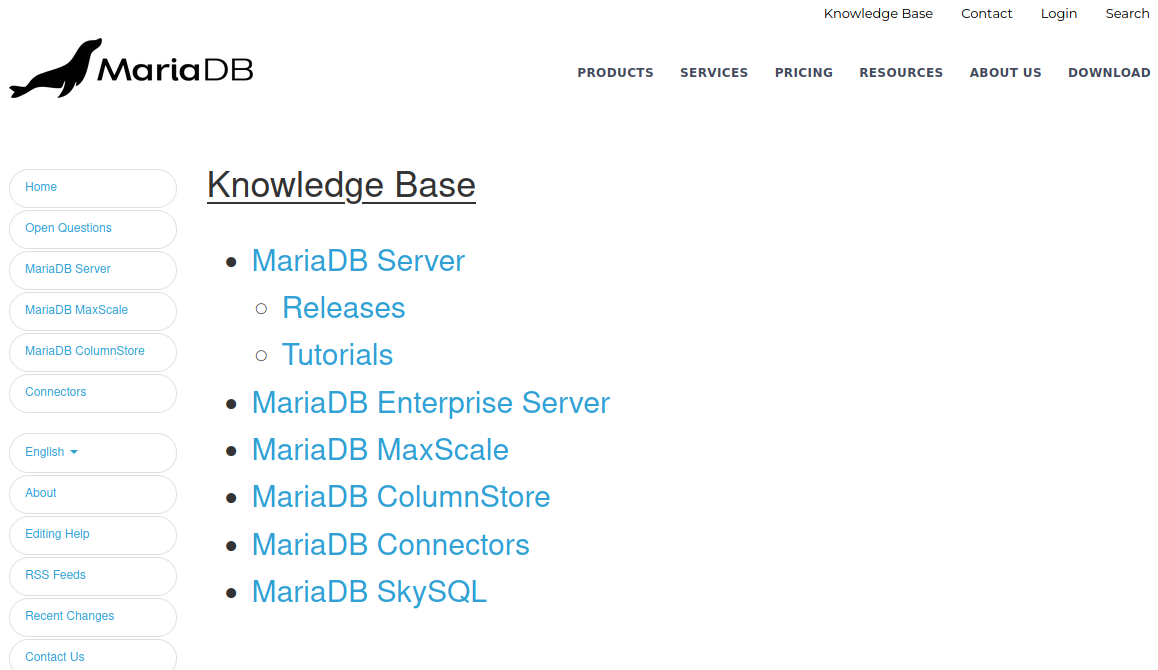
\includegraphics[scale=0.5]{images/maria1}
\end{figure}


%\addcontentsline{toc}{chapter}{SPRING}
\chapter{SPRING}
%\stepcounter{chapter}
El entorno de trabajo de Spring es popular y ampliamente usado entorno de trabajo de Java para construir aplicaciones web y de empresa. Su eje es la inyección de dependencias que provee flexibilidad para configurar de múltiple maneras, tales como XML, Commentarios, y configuraciones java. El entorno de trabajo Spring creció respondiendo a modernas necesidades de empresas como la seguridad, soporte para almacenamientos NoSql, manejo de GrandesDatos, proceso de lotes, integración con otros sistemas, etc. 

El entorno de trabajo Spring es flexible, tiene capacidad y fácil de uso transacciones de base de datos. simplifica la integración con otros entornos de trabajo, tiene una tecnología de punta para construir aplicaciones web en Modelo Vista Controlador. 
\section{Spring Boot}
Spring Boot es un entorno de trabajo que ayuda a desarrollar aplicaciones basados en Spring de forma fácil y rápida. Sus característica son:
\begin{itemize}
\item Iniciador de Spring Boot
\item Auto configuración
\item Manejo de configuración elegante
\item Actuador Spring Boot
\item Soporte de contenidos servlet y fácil de usar integrado
\end{itemize}

Spring Boot configura los componentes de la aplicación de forma automática, pero permitiendo invalidad los por defectos si requiere. 
Los pasos son:
\begin{enumerate}
\item Crear proyectos de Spring Boot basado en Maven y configurar las dependencias en el archivo \textit{pom.xml}
\item Configurar los recursos de datos/propiedades JPA en src/main/resources/aplication.properties.
\item Crear una entidad JPA llamada Usuario.java, una interfaz de repositorio de dato JPA Spring llamada RepositorioUsuario.java, y un controlador llamado HomeController.java
\item Crear un la vista para mostrar la lista de usuarios. 
\item Crea una una ClasePuntoEntrada Aplicacion.java con el método principal
\item Ejecutar la aplicación.java y dirigirse en el navegador al localhost:8080/
\end{enumerate}
Explicamos lo que está pasando:
\section{Fásil manejo de dependencias}
La dependencia llamada spring-boot-starter-*. este jala todas las librerías comunes al desarrollar aplicaciones Spring MVC tales como: spring-webmvc, jackson-json, validation-api, y tomcat. 
\section{Autoconfiguración}
Es su @EnableAutoConfiguration anote. 
\section{Soporte integrado de contenedor de servlet}
Se crea un clase simple comentado con (@SpringAplication), 

\subsection{Spring Initializr}
Para comenzar con el proyecto de Spring Boot se deber ir a la página \url{https://start.spring.io/}, configurar y pulsar generar. 
\begin{figure}[h]
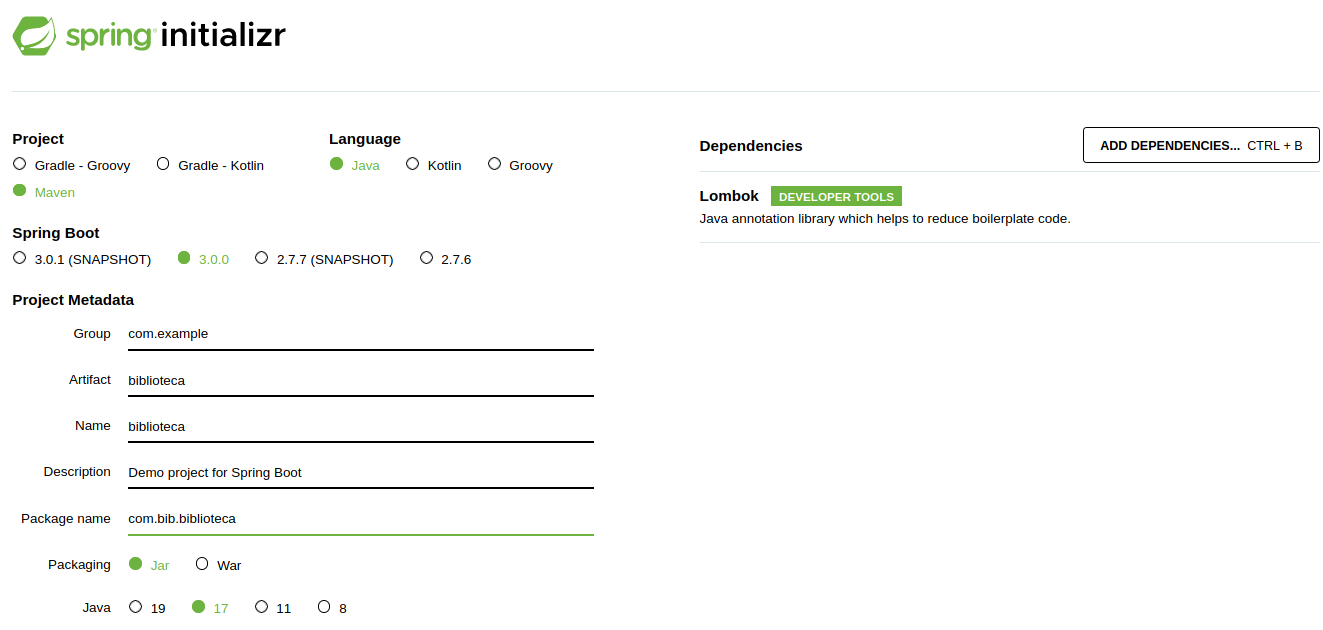
\includegraphics[scale=0.5]{images/spring1}
\caption{La configuración al iniciar un proyecto Spring Boot}
\end{figure}
Se verifica java para configurar. 
\begin{verbatim}
tomas@debian:~$ java --version
openjdk 17.0.4 2022-07-19
OpenJDK Runtime Environment (build 17.0.4+8-Debian-1deb11u1)
OpenJDK 64-Bit Server VM (build 17.0.4+8-Debian-1deb11u1, mixed mode, sharing)
\end{verbatim}

\section{Herramientas de desarrollo}




\addcontentsline{toc}{chapter}{IntelliJ IDEA}
\chapter*{IntelliJ IDEA}
\stepcounter{chapter}
IntelliJ IDEA es un Entorno de desarrollo Integrado (EDI) o Integrated Development Environment (IDE) para lenguajes JVM\footnote{Java
    Kotlin
    Scala
    Groovy
    Clojure
    Fantom
    Ceylon
    Jython
    JRuby
    Frege
    Xtend
    Golo
    Concurnaas
    Yeti } 
%https://www.spec-india.com/blog/jvm-languages
diseñado para maximizar la productividad del desarrollador. Hace la tareas rutinarias y repetitivas proporcionando un completado inteligente de código, análisis de código estático, refactoriza, y permite enfocarse en el lado brillante del desarrollo de software.

IntelliJ IDEA es multiplataforma, que provee una experiencia consistente en Windows, madOS, y Linux. 
Soportea múltiples lenguajes, herramientas, frameworks, y tecnologías. 

IntelliJ IDEA viene en tres ediciones:
\begin{itemize}
\item \textbf{IntelliJ IDE Ultimate}: Es la edición comercial para JVM, web, y desarrollo corporativo. Incluye todas las características de la edición Community, soporta una variedad de frameworks al lado des servidor así como del front-end, servidor de aplicaciones, integración con base de datos y soporte de herramientas y mucho mas. 
\item \textbf{IntelliJ IDEA Community Edition:} Es la edición gratuita basado en Open-source para JVM y desarrollo Android.
\item \textbf{IntelliJ IDEA Edu:} Es la edición libre con lecciones incorporadas para aprender Java, Kotlin, y Scala. Tiene características especiales para profesores para crear su propio curso y gestionar el proceso de aprendizaje. 
\end{itemize}

La interfaz de usuario sigue el contexto y trae herramientas necesarias de forma automática para ayudar a minimizar el riesgo de interrumpir el flujo del desarrollador. 

Lo mejor de IntelliJ IDEA es su configurabilidad, es decir se puede configurar cualquier cosa. Por ejemplo el color del fuente, salida de la consola, depurador, resultados de búsqueda, etc. 

Tiene atajos de teclado para toda acción,casi, incluyendo la selección y intercambiar el editor y varias herramientas de windows. 

Uno de los más útiles accesos por teclado es el doble shift que abre el dialogo \textbf{Buscar en todo}, buscará entre todos los archivos, clases, y símbolos que pertenecen al proyecto e incluso entre las acciones del IDE. 
\begin{figure}[h]
\centering
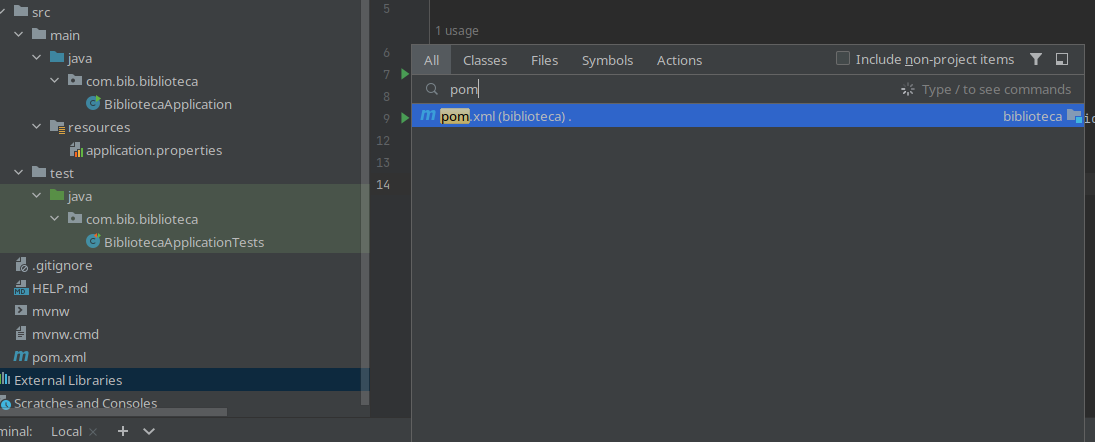
\includegraphics[width=10cm]{images/idea3}
\caption{Ventana de dialogo de buscar en todo}
\end{figure}
Puedes usar también esta acción para abrir cualquier herramienta de ventana. 

\section{Asistente al codificar}
El completado de código ayuda en la velocidad el proceso de codificar. El completado básico ayuda a completar los nombres de las clases, métodos, campos, y palabras reservadas.

El \textbf{completado inteligente} sugiere el más relevante símbolo aplicable en el contexto actual, cuando IntelliJ IDEA puede determinar el tipo apropiado. 
\section{Refactorización}
IntelliJ IDEA ofrece un comprensible conjunto de refactorización de código que permite una productividad significativa. Por ejemplo cuando renombra una clase, el IDE ayuda a actualizar todas las referencias a esa clase, sin siquiera seleccionar y solo requiere confirmación. 
\section{Terminal}
IntelliJ IDEA viene con terminal incorporado para trabajar con comandos de shell desde el IDE. Por ejemplo permite ejecutar comandos de Git. Soporta cmd.exe, bash, sh, etc. 
\section{Herramientas de construcción}
IntelliJ IDEA viene con un completo y funcional Gradle y Maven integrado que permite automatizar el proceso de construcción, empaquetado, correr pruebas, despliegue, y otras actividades. IntelliJ IDEA detecta y descarga automaticamente todo los repositorios requeridos y plugins, y no requiere usted configurar nada. 
\section{Control de Versiones}
IntelliJ IDEA está integrado con herramientas de control de versiones como, Git, Mercurial, Perforce, y Subversion. 
\section{Requerimientos del sistema e instalación}
Se puede ir a la siguiente dirección \url{https://www.jetbrains.com/idea/download/#section=linux}
\begin{figure}[h]
\centering
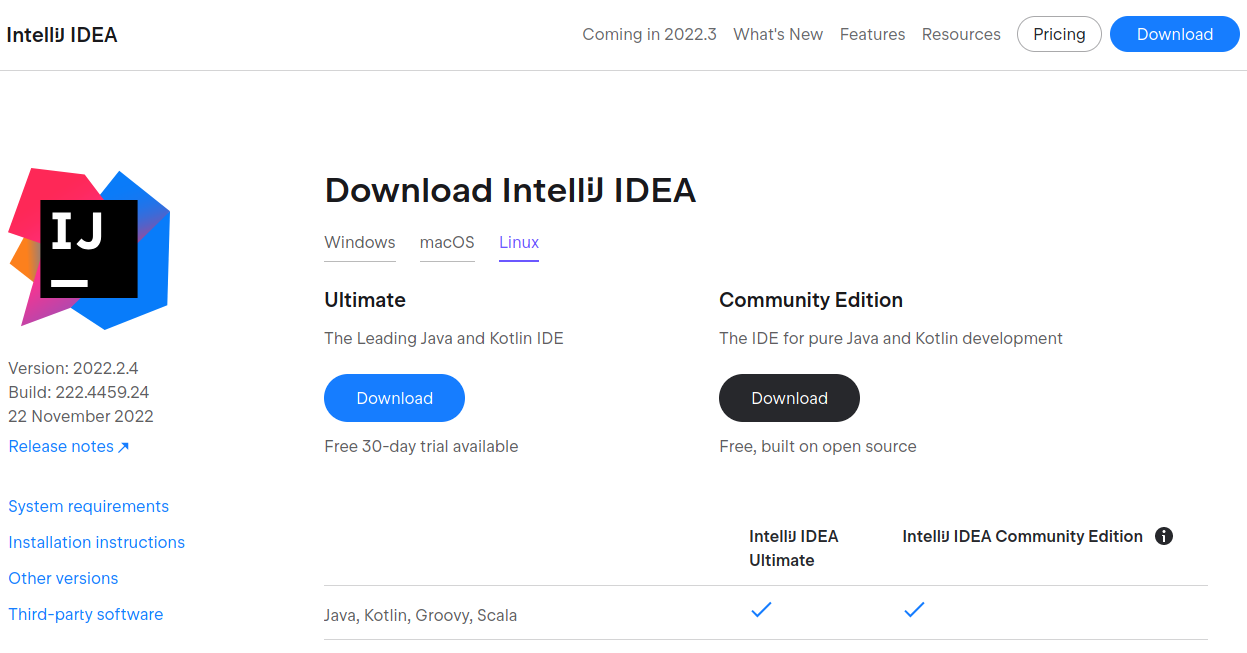
\includegraphics[width=10cm]{images/idea1}
\caption{Sección de descarga para Linux}
\end{figure}
En Linux cualquier distribución que soporte Gnome, KDE, o Unity DE puede soportarlo.
También se puede instalar por linea de comando:
\begin{verbatim}
sudo snap install intellij-idea-community --classic
or
sudo snap install intellij-idea-ultimate --classic

or
sudo snap install intellij-idea-educational --classic
\end{verbatim}
En el caso para el proyecto fue solo necesario descargar el comprimido en .tar, descomprimir y ejecutarlo por un comando el archivo idea.sh en la carpeta done se descomprimió:
\begin{figure}[h]
\centering
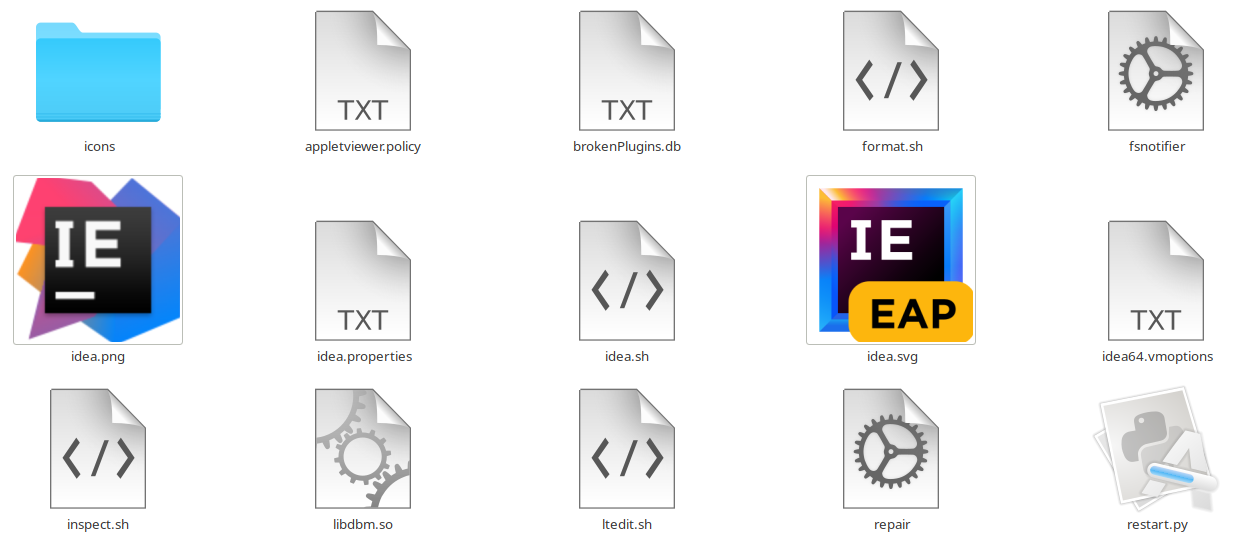
\includegraphics[width=10cm]{images/idea4}
\caption{Carpeta bin de la carpeta descomprimida}
\end{figure}

Una vez descomprimido el inicializado de Spring Boot y abierto en el editor IntelliJ IDEA no muestra lo siguiente:
\begin{figure}[h]
\centering
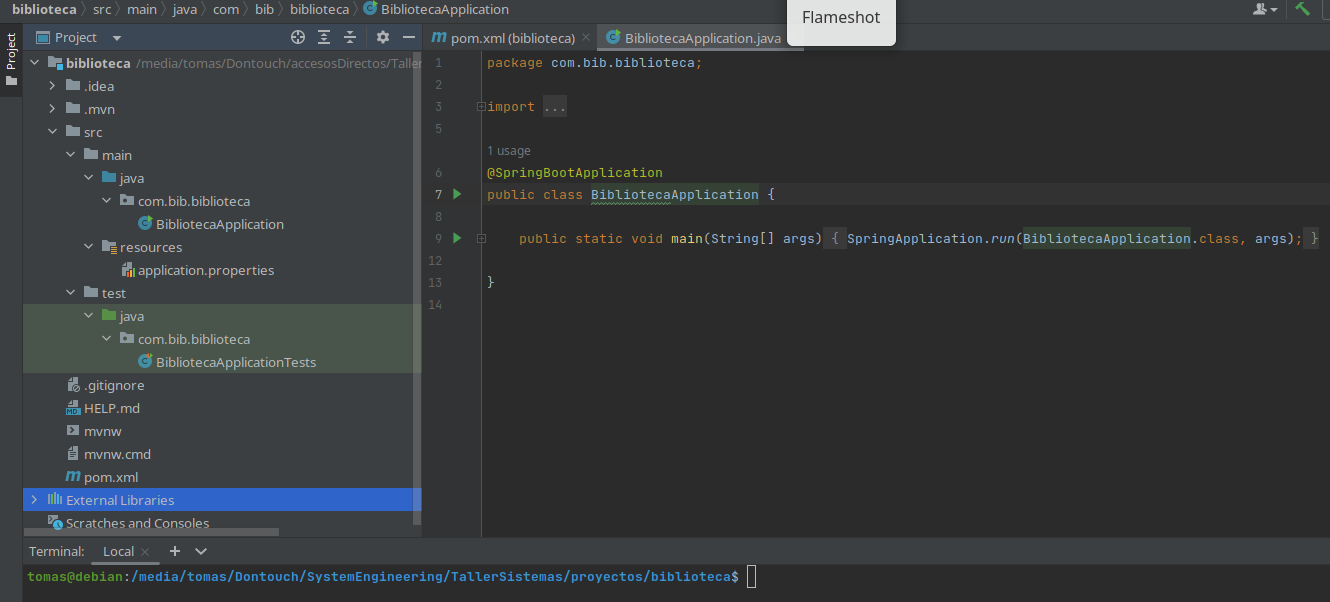
\includegraphics[width=10cm]{images/idea2}
\caption{El proyecto abierto por primera vez}
\end{figure}

\chapter{DBEAVER}
DBeaver is un gestor de base de datos universal y profesional. Es capaz de manipular los datos, crear reportes analíticos basado en registros desde diferentes almacenes de base de datos, y exportar la información en un formato apropiado. 

DBeaver ofrece:
\begin{itemize}
\item Interfaz de usuario cuidadosamente diseñado e implementado.
\item Soporte de datos en la nube.
\item Soporte estandar para seguridad empresarial
\item Capacidad de trabajar con varias extensiones para integración con Excel, Git y otros
\item Soporte multiplataforma
\end{itemize}

DBeaver se utilizó como herramienta de base de datos, se descargó de su página oficial \url{https://dbeaver.io/}
se conenecto con dbeaver en puerto 3306 desde debian. La base de datos se llama DBCUERVO
Para no tener error al conectar con la base de datos se realiza lo siguiete. 
\begin{enumerate}
\item sudo service mysqld stop
\item sudo netstat -nap | grep :80 
\item sudo kill 1433
\item /opt/lampp/lampp stop
\item /opt/lampp/lampp start
\end{enumerate}
El comando sudo service mysqld stop es necesario para detener mysql y luego en seguida con el comando  sudo netstat -nap  grep :80 se busca que servidor está en ejecución en puerto 80 como sigue tcp6       0      0 :::80                   :::*                    LISTEN      1433/apache2    en este caso el proceso 1433 se debe detener con sudo kill 1433
y en seguida con el comando sudo /opt/lampp/lampp start se inicia de nuevo el servidor y tendremos el siguiente resultado:
\begin{verbatim}
Starting XAMPP for Linux 8.1.10-0...
XAMPP: Starting Apache...fail.
XAMPP:  Another web server is already running.
XAMPP: Starting MySQL...ok.
XAMPP: Starting ProFTPD...ok.
\end{verbatim}
Aquí se puede ver que Apache no se pudo iniciar porque no ejecutamos el paso 3, repitiendo correctamente es decir desocupando el puero 80 ya no da lo siguiente:
\begin{verbatim}
Starting XAMPP for Linux 8.1.10-0...
XAMPP: Starting Apache...ok.
XAMPP: Starting MySQL...already running.
XAMPP: Starting ProFTPD...already running.
\end{verbatim}
Una vez hecho esto se puede iniciar con el gestor de base de datos DBeaver y no da error al conectar. Estos pasos siempre se los hace cada que inicia la computadora debe haber una manera de que el servidor esté corriendo siempre pero por motivos de tiempo no se pudo averiguar. 
\chapter{SWAGGER}
Es un conjunto de herramientas para desarrolladores API (aplication program interface) proveido por la compañía de tecnología \textit{SmartBear Software}. 

Fue creado en 2011 por Tony Tam por necesidad
\section{Swagger UI}
La interfaz de usuario de Swagger permite que cualquier persona, visualice e interactúe con los recursos de la API . Se genera automáticamente a partir de su especificación OpenAPI (anteriormente conocida como Swagger), con la documentación visual que facilita la implementación de back-end y el consumo del lado del cliente.


    

\chapter{Diccionario de datos}
% inicia dic datos%%%%%%%%%%%%%%%%%%%

%----------------------------------------DOCUMENTO--------------------------

\begin{table}[h]
\begin{tabular}{lllp{10cm}}
\multicolumn{3}{l}{Nombre del archivo: Documento} & \multicolumn{1}{l}{Fecha de creación \today}\\
\multicolumn{4}{l}{Descripción: Cualquier objeto digital que requiera el estudiante} \\ \hline
\multicolumn{1}{c}{\textbf{Campo}} & \multicolumn{1}{c}{\textbf{Tamaño}} & \multicolumn{1}{c}{\textbf{Tipo de dato}} & \multicolumn{1}{c}{\textbf{Descripción}} \\ \hline

idDoc   & 6   & Numérico    & Clave única de registro de documento  \\
titulo  & 500  & Caracter   & Título del documento digital \\
lenguaje & 20  & Caracter   & Lengua en el que está el documento \\
ocupa    & 5   & Numérico   & Cantidad que ocupa en un dispositivo de almacenamiento  \\
descripcion   & 200  & Caracter  & Breve descripción del documento  \\ 
fechaReg      & x    & Date      & Es la fecha en que se registró el documento         \\ 
\hline
\multicolumn{3}{l}{Relaciones: idDocumento con idAutor} & \multicolumn{1}{l}{Campos clave: idDocumento}          
\end{tabular}
\end{table}
%--------------------------- ACADÉMICO--------------------------
\begin{table}[h]
\begin{tabular}{lllp{10cm}}
\multicolumn{3}{l}{Nombre del archivo: Académico} & \multicolumn{1}{l}{Fecha de creación: \today}\\
\multicolumn{4}{l}{Descripción: Base de datos que contiene documentos académicos o científicos} \\ \hline
\multicolumn{1}{c}{\textbf{Campo}} & \multicolumn{1}{c}{\textbf{Tamaño}} & \multicolumn{1}{c}{\textbf{Tipo de dato}} & \multicolumn{1}{c}{\textbf{Descripción}} \\ \hline

idAcademico   & 6   & Numérico    & Clave única de registro de documento académico  \\
doi  & 300  & Caracter   & Identificador digital de documento \\
paginas  & x  & Numérico   & Número de páginas que tiene el documentos académico \\
ano & 4  & numérico   & Es el año que se publicó el documento\\
\hline
\multicolumn{3}{l}{Relaciones: idAcademico con idDocumento} & \multicolumn{1}{l}{Campos clave: idAcademico y doi}          
\end{tabular}
\end{table}
%%----------------------------------------LIBRO--------------------------
\begin{table}[h]
\begin{tabular}{lllp{10cm}}
\multicolumn{3}{l}{Nombre del archivo: Libro} & \multicolumn{1}{l}{Fecha de creación: \today}\\
\multicolumn{4}{l}{Descripción: Base de datos que contiene libros} \\ \hline
\multicolumn{1}{c}{\textbf{Campo}} & \multicolumn{1}{c}{\textbf{Tamaño}} & \multicolumn{1}{c}{\textbf{Tipo de dato}} & \multicolumn{1}{c}{\textbf{Descripción}} \\ \hline

idLibro   & 18   & Numérico    & Clave única de registro de documento académico  \\
edicion    & 3  & Numérico   & Es el número de edición del libro \\
Editorial  & 20  & Caracter   & Es el editorial publicador del libro \\
\hline
\multicolumn{3}{l}{Relaciones:idLibro con idAcademico} & \multicolumn{1}{l}{Campos clave: idLibro}          
\end{tabular}
\end{table}
%----------------------------------------ARTICULO--------------------------
\begin{table}[H]
\begin{tabular}{lllp{10cm}}
\multicolumn{3}{l}{Nombre del archivo: Articulo} & \multicolumn{1}{l}{Fecha de creación: \today}\\
\multicolumn{4}{l}{Descripción: Base de datos que contiene artículos} \\ \hline
\multicolumn{1}{c}{\textbf{Campo}} & \multicolumn{1}{c}{\textbf{Tamaño}} & \multicolumn{1}{c}{\textbf{Tipo de dato}} & \multicolumn{1}{c}{\textbf{Descripción}} \\ \hline

idArticulo   & 18   & Numérico    & Clave única de registro artículos  \\
revista    & 200  & Caracter   & Es la revista que publica el artículo \\
\hline
\multicolumn{3}{l}{Relaciones: idLibro con idDocumento} & \multicolumn{1}{l}{Campos clave: idArticulo}          
\end{tabular}
\end{table}
%----------------------------------------AUTOR--------------------------
\begin{table}[H]
\begin{tabular}{lllp{10cm}}
\multicolumn{3}{l}{Nombre del archivo: Autor} & \multicolumn{1}{l}{Fecha de creación: \today}\\
\multicolumn{4}{l}{Descripción: Base de datos que contiene autores} \\ \hline
\multicolumn{1}{c}{\textbf{Campo}} & \multicolumn{1}{c}{\textbf{Tamaño}} & \multicolumn{1}{c}{\textbf{Tipo de dato}} & \multicolumn{1}{c}{\textbf{Descripción}} \\ \hline

idAutor   & 18   & Numérico    & Clave única de registro de un autor  \\
nombreAutor    & 200  & Caracter   & Es el nombre del autor \\
\hline
\multicolumn{3}{l}{Relaciones: idAutor con idDocumento} & \multicolumn{1}{l}{Campos clave: idAutor}          
\end{tabular}
\end{table}

\chapter{Descripción de API REST}

\begin{table}[H]
\centering
\begin{tabular}{|lp{10cm}|} \hline
Metodo http & GET \\%, POST, PUT y DELETE
url   &  \url{http://kuerva:2295/org/biblioteca2295/almacen}\\
Descripción & Es servicio lista todos los libros de la biblioteca digital 2295.\\ \hline
\end{tabular}
\end{table}

%\part{Testing}
%\chapter*{TESTING O PRUEBAS}
%Se ve la funcionalida y la integración, tiempo de respuesta, afección al hardware, que no sea pesado





%\chapter{apuntito}
\section{INTEGRANTES DEL DESARROLLO}
El analista, el líder del proyecto, diseño UX, arquitecto de software, tester, programador, analista programador.

El arquitecto y el UX realizan la interfaz. 
\section{Flutter}
En la cronología de evolución de software, fluter que es un kit de desarrollo de google que utiliza Dart se puede hacer desarrollo multiplataforma. Estamos ahora en la época de ORM


\appendix
%\chapter{GLOSARIO}
\begin{itemize}
\item \textbf{Documento u objeto digital} Cualquier objeto, como libros, audio, imágenes, simuladores
%\item \textbf{BPMN}Busness process managemen
\item \textbf{OCR: }Optical Character Recognition, Es el proceso de producicr una representacion digital de un texto de una imagen.
\item \textbf{OMR: }Optical Music Recognition, análogo del OCR para música.
\item \textbf{PDF}: Portable Document Format, 
\item \textbf{RTF}: Rich Text Format
\end{itemize}




\bibliographystyle{apalike}
\bibliography{ref}



\end{document}

